
\section{Genotype calling}

%%%%%%%%%%%%%%%%%%%%%%%%%%%%%%%%%%%%%%%%%%%%%%%%%%%

\frame{\frametitle{Genotype calling}

	\begin{columns}
	
    	\column{0.6\textwidth}   

		\begin{center}
			\begin{tabular}{c | c}
			Genotype & Likelihood (log10)\\
    		\hline
	    	AA & -2.49\\
    		AC & -3.38\\
    		AG & -1.22\\
    		AT & -3.38\\
            CC & -9.91\\
            CG & -7.74\\
            CT & -9.91\\
            GG & -7.44\\
            GT & -7.74\\
            TT & -9.91\\
        	\hline
			\end{tabular}
       	\end{center}

		\column{0.4\textwidth}

		AAAG \& $\epsilon=0.01$

		\begin{block}{}
			What is the genotype here?
		\end{block}

	\end{columns}


}

%%%%%%%%%%%%%%%%%%%%%%%%%%%%%%%%%%%%%%%%%%%%%%%%%%%

\frame{\frametitle{Genotype calling}

	\begin{columns}
	
    	\column{0.6\textwidth}   

		\begin{center}
			\begin{tabular}{c | c}
			Genotype & Likelihood (log10)\\
    		\hline
	    	AA & -2.49\\
    		AC & -3.38\\
    		\textbf{AG} & \textbf{-1.22}\\
    		AT & -3.38\\
            CC & -9.91\\
            CG & -7.74\\
            CT & -9.91\\
            GG & -7.44\\
            GT & -7.74\\
            TT & -9.91\\
        	\hline
			\end{tabular}
       	\end{center}

		\column{0.4\textwidth}

		AAAG \& $\epsilon=0.01$

		What is the genotype? AG.

		\begin{block}{Maximum Likelihood}
			The simplest genotype caller: choose the genotype with the highest likelihood.
		\end{block}

	\end{columns}


}

%%%%%%%%%%%%%%%%%%%%%%%%%%%%%%%%%%%%%%

\frame{\frametitle{Major and minor alleles}

	\begin{block}{Likelihood function}
		\begin{equation*}
			P(D|G=A) = \sum_{i=1}^R \log L_{A_j,i}
		\end{equation*}
	\end{block}

	AAAG \& $\epsilon=0.01$

	\begin{center}
		\begin{tabular}{c | c}
		Allele & Likelihood\\
    	\hline
	    \textbf{A} & \textbf{-2.49}\\
    	C & -3.38\\
    	\textbf{G} & \textbf{-1.22}\\
    	T & -3.38\\
        \hline
		\end{tabular}
	\end{center}

	We can reduce the genotype space to 3 entries (from 10).
    
}    
    
%%%%%%%%%%%%%%%%%%%%%%%%%%%%%%%%%%%%%%

\frame{\frametitle{Genotype calling}

	AAAG \& $\epsilon=0.01$ \& A,G alleles

	\begin{center}
		\begin{tabular}{c | c}
		Genotype & Likelihood\\
    	\hline
	    AA & -5.73\\
    	AG & -2.80\\
    	GG & -17.12\\
        \hline
		\end{tabular}
	\end{center}

	Examples varying qualities and reads...
    
}   

%%%%%%%%%%%%%%%%%%%%%%%%%%%%%%%%%%%%%%%%%%%

\frame{\frametitle{Genotype likelihood ratio}

	\begin{equation*}
		\log_{10} \frac{L_{G(1)}}{L_{G(2)}} > t
	\end{equation*}

	i.e. $t=1$ meaning that the most likely genotype is 10 times more likely than the second most likely one

	Pros and cons?
 	\begin{itemize}
 	\item Yes:
    \item No:
 	\end{itemize}

}

%%%%%%%%%%%%%%%%%%%%%%%%%%%%%%%%%%%%%%%%%%%

\frame{\frametitle{Genotype likelihood ratio}

	\begin{equation*}
		\log_{10} \frac{L_{G(1)}}{L_{G(2)}} > t
	\end{equation*}

	i.e. $t=1$ meaning that the most likely genotype is 10 times more likely than the second most likely one

	Pros and cons?
 	\begin{itemize}
 	\item Yes: genotype are called with higher \textbf{confidence}
    \item No: more \textbf{missing} data
 	\end{itemize}

}


%%%%%%%%%%%%%%%%%%%%%%%%%%%%%%%%%%%%%%%%%%%%%%%%%%%%%

\frame{
\frametitle{Statistical thinking}

\begin{figure}[!ht]
\centering
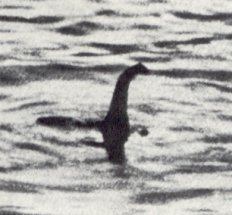
\includegraphics[width=4cm]{Pics/LochNessMonster.jpg}
\caption{Nessie, the Loch Ness Monster. True or fake?}
\end{figure}

}

%%%%%%%%%%%%%%%%%%%%%%%%%%%%%%%%%%%%%%%%%%%%%%%%%%%%%%%%

\frame{
\frametitle{Statistical thinking}

\begin{itemize}
\item $T = \{0,1\}$, whether I tell you I saw Nessie or not.
\item $N = \{0,1\}$, whether Nessie exists (I saw it) or not.
\end{itemize}

\begin{block}{Questions}
\begin{itemize}
\item What are $p(T=1|N=1)$ and $p(T=1|N=0)$?
\item What is a Maximum Likelihood Estimate of $N$?
\end{itemize}
\end{block}

}

%%%%%%%%%%%%%%%%%%%%%%%%%%%%%

\frame{
\frametitle{Statistical thinking}

Our inference on $N$ is driven solely by our observations, given by our likelihood function.

\begin{figure}[!ht]
\centering
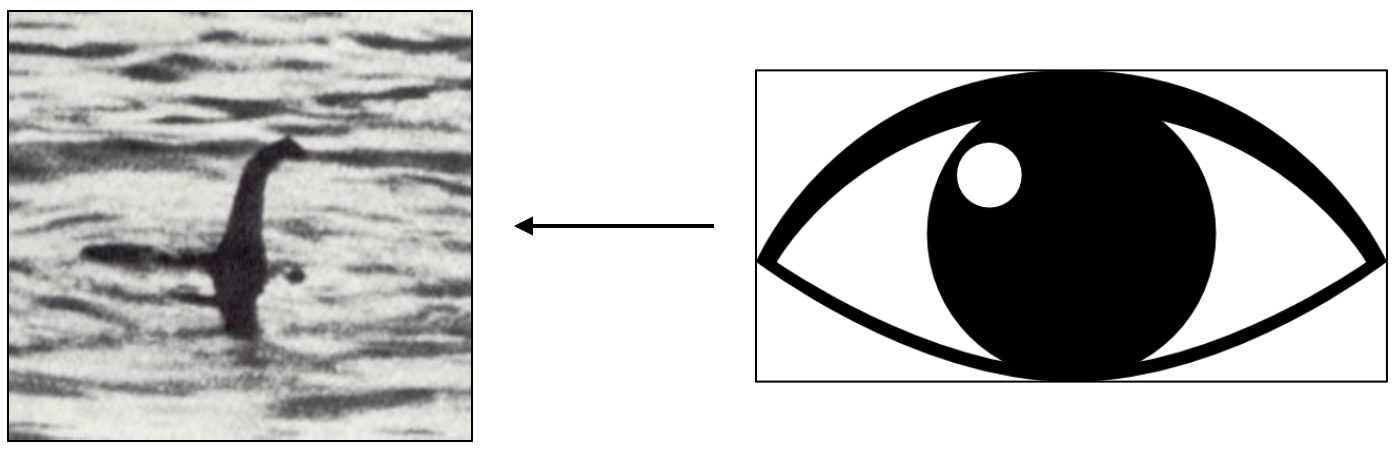
\includegraphics[width=5cm]{Pics/EyeOnly.png}
\caption{The eye: a "likelihood" organ.}
\end{figure}

}

%%%%%%%%%%%%%%%%%%%%%%%%%%%%%

\frame{
\frametitle{Statistical thinking}

In real life we take many decisions based not only on what we observe but also on some believes of ours.

\begin{figure}[!ht]
\centering
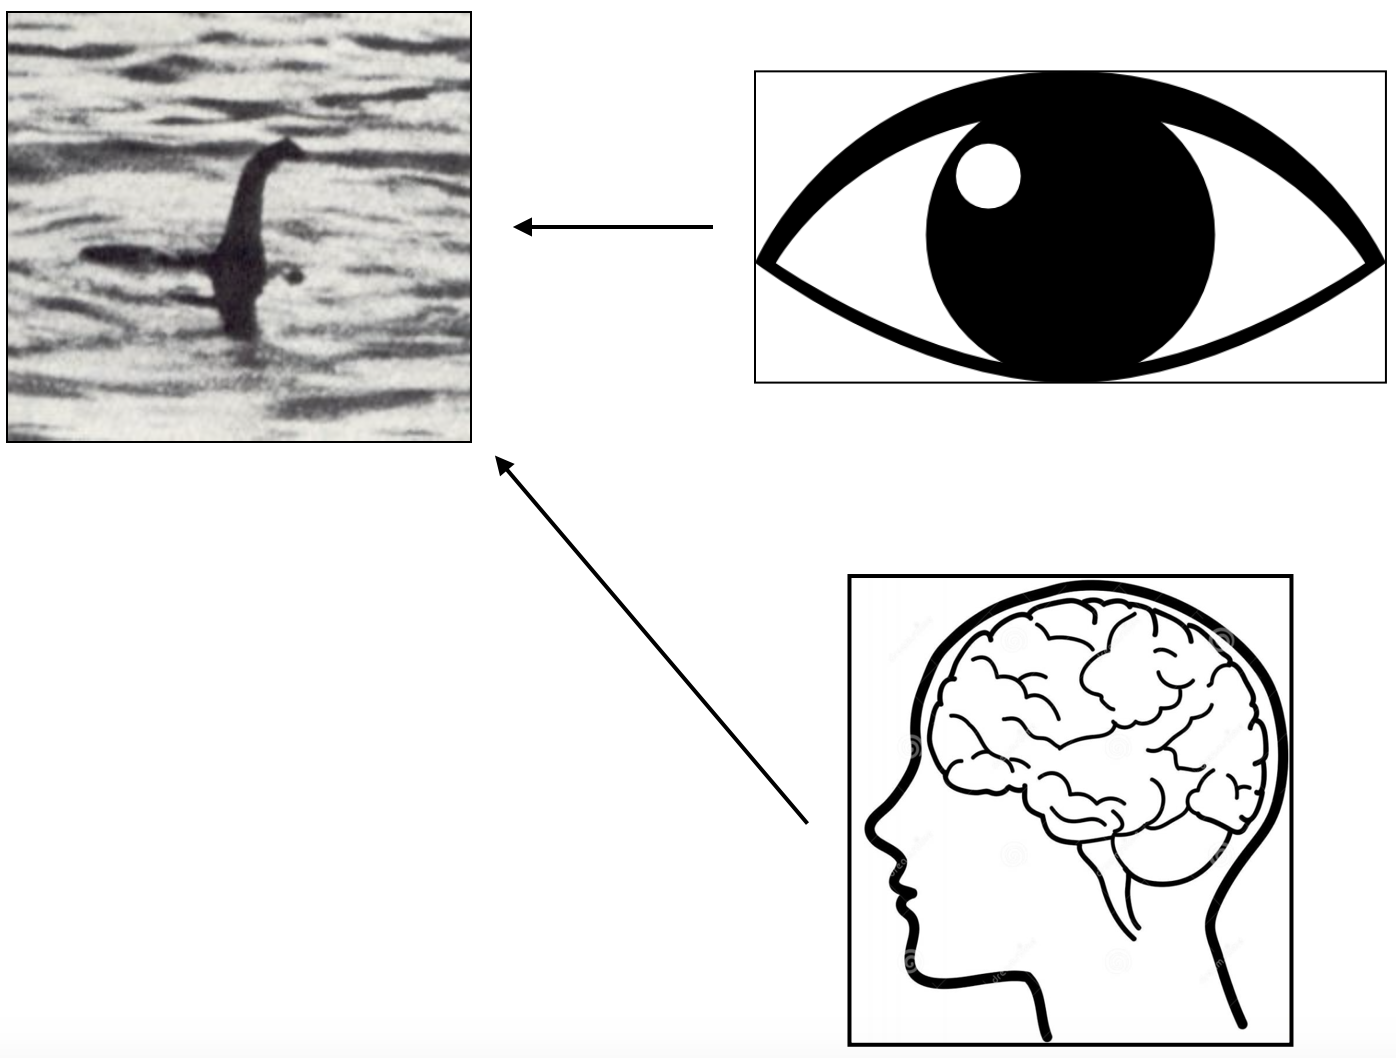
\includegraphics[width=5cm]{Pics/EyeBrain.png}
\caption{The brain: a "non-likelihood" organ.}
\label{Fig:EyeBrain}
\end{figure}

}

%%%%%%%%%%%%%%%%%%%%%%%%%%%%%%%%%%%%%%%%%%%%%%%%

\frame{
\frametitle{Bayesian thinking}

\begin{itemize}
\item with "eyes only" our intuition is that $p(N|T) \approx p(T|N)$
\item with "the brain" our intuition is that $p(N|T) \approx p(T|N)p(N)$
\end{itemize}

Our "belief" expresses the probability $p(N)$ \textbf{unconditional} of the data.

\begin{block}{Question}
How can we define $p(N)$?
\end{block}

}

%%%%%%%%%%%%%%%%%%%%%%%%%%%%%%%%%%%%%%%%%%%%%%%%%

\frame{
\frametitle{Bayesian thinking}

\begin{block}{}
The "belief" function $p(N)$ is called \textbf{prior probability} and the joint product of the likelihood $p(T|N)$ and the prior is proportional to the \textbf{posterior probability} $p(N|T)$.
\end{block}

\begin{block}{}
The use of posterior probabilities for inferences is called Bayesian statistics.
\end{block}

}

%%%%%%%%%%%%%%%%%%%%%%%%%%%%%%%%%%%%%%%%%%%%%%%%%

\frame{
\frametitle{Statistical inference}

If $D$ is the data and $\theta$ is your unknown parameter, then
\begin{itemize}
\item the frequentist conditions on parameters and integrates over the data, $p(D|\theta)$,
\item the Bayesian conditions on the data and integrates over the parameters, $p(\theta|D)$.
\end{itemize}

}

%%%%%%%%%%%%%%%%%%%%%%%%%%%%%%%%%%

\frame{
\frametitle{Statistical inference}

\begin{block}{Bayesian \textit{vs.} Likelihoodist}
\begin{itemize}
\item we derive "proper" probability distributions of our parameters rather than deriving a point estimate;
\item a probability is assigned to a hypothesis rather than a hypothesis is tested;
\item we can "accept" the null hypothesis rather than "fail to reject" it;
\item parsimony imposed in model choice rather than correcting for multiple tests.
\end{itemize}
\end{block}

}

%%%%%%%%%%%%%%%%%%%%%%%%%%%%%%%%%%%%%%%%

\frame{
\frametitle{Bayesian inference}

\begin{figure}[!ht]
\centering
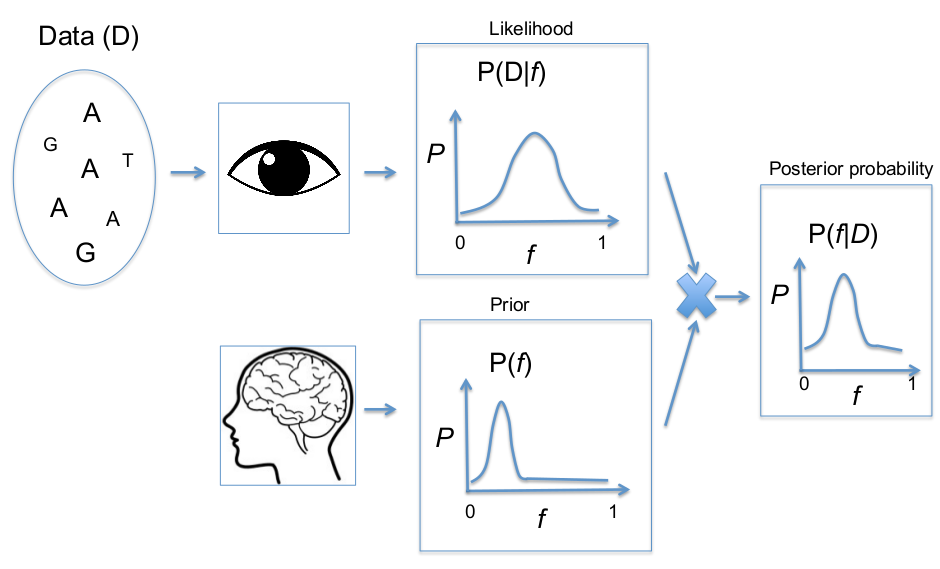
\includegraphics[width=7cm]{Pics/bayesian.png}
\end{figure}

}


%%%%%%%%%%%%%%%%%%%%%%%%%%%%%%

\frame{
\frametitle{Bayesian concepts}

\begin{block}{Bayes' Theorem}

\begin{equation}
p(\vec{\theta}|\vec{y}) = \frac{f(\vec{y}|\vec{\theta})\pi(\vec{\theta})}{m(\vec{y})} = \frac{f(\vec{y}|\vec{\theta})\pi(\vec{\theta})}{\int f(\vec{y}|\vec{\theta}) d\vec{\theta}}
\end{equation}
\end{block}

\begin{itemize}
\item $\vec{\theta}$ is not a fixed parameter but a random quantity with prior distribution $\pi(\vec{\theta})$
\item $p(\vec{\theta}|\vec{y})$ is the posterior probability distribution of $\vec{\theta}$
\item $\int p(\vec{\theta}|\vec{y})d\vec{\theta}=1$
\end{itemize}

}

%%%%%%%%%%%%%%%%%%%%%%%%%%%%%%%%%%%%%%%%%%%%%

\frame{
\frametitle{Genotype posterior probability}

	AAAG \& $\epsilon=0.01$ \& A,G alleles

	\begin{center}
		\begin{tabular}{c | c | c | c}
		Genotype & Likelihood (log) & Prior & Posterior\\
    	\hline
	    AA & -5.73 & 1/3 & 0.05\\
    	AG & -2.80 & 1/3 & 0.95\\
    	GG & -17.12 & 1/3 & ~0\\
        \hline
		\end{tabular}
	\end{center}

	Only call genotypes if the largest probability is above a certain threshold (e.g. 0.95).

}

%%%%%%%%%%%%%%%%%%%%%%%%%%%%%%%%%%%%%%%%%%%%%

\frame{
\frametitle{Genotype posterior probability}

	AAAG \& $\epsilon=0.01$ \& A,G alleles

	\begin{center}
		\begin{tabular}{c | c | c | c}
		Genotype & Likelihood (log) & Prior & Posterior\\
    	\hline
	    AA & -5.73 & 1/3 & 0.05\\
    	AG & -2.80 & 1/3 & 0.95\\
    	GG & -17.12 & 1/3 & ~0\\
        \hline
		\end{tabular}
	\end{center}

	Only call genotypes if the largest probability is above a certain threshold (e.g. 0.95).

}

%%%%%%%%%%%%%%%%%%%%%%%%%%%%%%%%%%%%%%%%%%%%%%%%%

\frame{
\frametitle{Genotype posterior probability}

	AAAG \& $\epsilon=0.01$ \& A,G alleles \& \textbf{A is the reference allele}

	$P(AA) > P(AG) > P(GG)$

	\begin{center}
		\begin{tabular}{c | c | c | c}
		Genotype & Likelihood (log) & Prior & Posterior\\
    	\hline
	    AA & -5.73 & 0.80 & 0.22\\
    	AG & -2.80 & 0.15 & 0.78\\
    	GG & -17.12 & 0.05 & ~0\\
        \hline
		\end{tabular}
	\end{center}
    

	The reference allele is just one of the possible alleles, often chosen arbitrarily: why give it so much weight?

}

%%%%%%%%%%%%%%%%%%%%%%%%%%%%%%%%%%%%%%%%%%%%%%%%%

\frame{
\frametitle{Genotype posterior probability}

	AAAG \& $\epsilon=0.01$ \& A,G alleles \& \textbf{$f(A)=0.7$} from a reference panel

	$P(AA)=?$;
    $P(AG)=?$;
    $P(GG)=?$

	\begin{center}
		\begin{tabular}{c | c | c | c}
		Genotype & Likelihood (log) & Prior & Posterior\\
    	\hline
	    AA & -5.73 & 0.49 & 0.06\\
    	AG & -2.80 & 0.42 & 0.94\\
    	GG & -17.12 & 0.09 & ~0\\
        \hline
		\end{tabular}
	\end{center}

	If the assumption of HWE can be reasonably met.

}

%%%%%%%%%%%%%%%%%%%%%%%%%%%%%%%%%%%%%%%%%%%%%%%%%

\frame{\frametitle{Empirical Bayesian inference}

\begin{figure}[!ht]
\centering
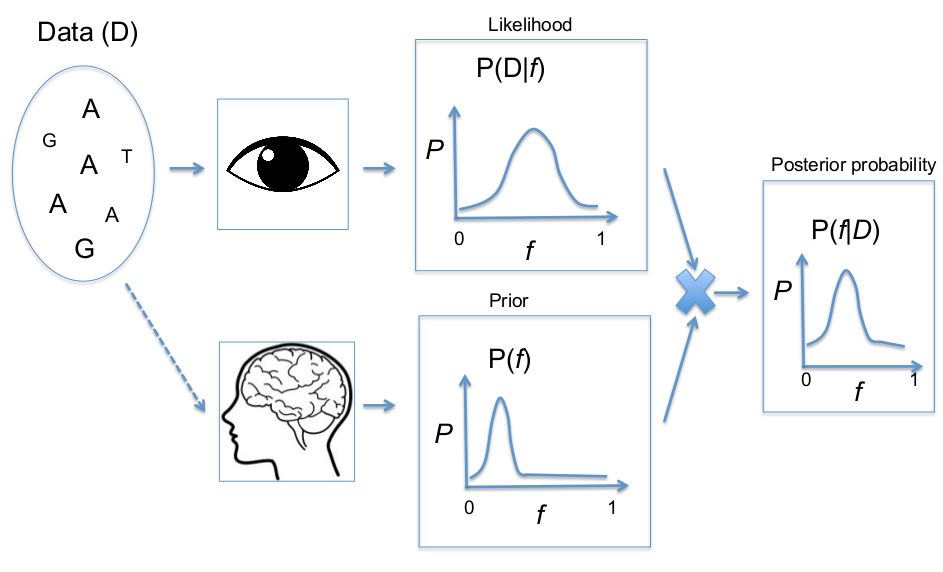
\includegraphics[width=8cm]{Pics/statEB.png}
\end{figure}



}

%%%%%%%%%%%%%%%%%%%%%%%%%%%%%%%%%%%%%%%%%%%%%%%%%

\frame{\frametitle{Genotype posterior probability}

	AAAG \& $\epsilon=0.01$ \& A,G alleles \& \textbf{$f(A)=0.6$} from the data itself

	$P(AA)=?$;
    $P(AG)=?$;
    $P(GG)=?$

	\begin{center}
		\begin{tabular}{c | c | c | c}
		Genotype & Likelihood (log) & Prior & Posterior\\
    	\hline
	    AA & -5.73 & 0.49 & 0.04\\
    	AG & -2.80 & 0.42 & 0.96\\
    	GG & -17.12 & 0.09 & ~0\\
        \hline
		\end{tabular}
	\end{center}

	\begin{itemize}
	\item if the assumption of HWE can be reasonably met
    \item if you have enough samples to have a robust estimate of the allele frequencies
	\end{itemize}

	How can we estimate allele frequencies?
	

}


